\section{Evaluation}

In diesem Kapitel wird untersucht, ob und wie der umgesetzte Prototyp den Anforderungen an das System gerecht wird. Grundlage der Untersuchung ist das Testen des Prototyps. Ähnlich wie die Anforderungsanalyse, erfolgt auch die Evaluation für die Abstraktionsebenen Kontextebene, Systemebene und technische Ebene. Auf Basis dieser Evaluationen wird schließlich eine passende Handlungsempfehlung für den Anwendungsfall gegeben. 

% Kontextebene
\subsection{Evaluation auf Kontextebene}
In der Kontextebene wurden Anforderungen an das System gestellt, welche sich aus den Einflussfaktoren im Systemkontext ergeben. Besonders die Probleme im Zusammenhang mit der Branche der Energiewirtschaft bilden die Kernanforderungen an das System (s. Anhang \ref{anfkontext}). Die sich daraus ergebenden funktionalen Anforderungen (K-FA-1) können im Großen und Ganzen als erfüllt betrachtet werden. Angefordert war es, dem Nutzer die Einsicht auf den digitalen Zwilling einer Anlage zu gewähren, einschließlich der Anzeige von Messwerten, Standorten und prädiktiven Informationen. Mit Betrachtung der Abbildungen \ref{thingpage}, \ref{landing}, \ref{detailoverview} und \ref{thingdetail} scheinen die Anforderungen erfüllt: Die Anlage wird auf der Startseite auf einer Landkarte verortet, die Übersicht über den Zustand liefert Bewertungen des Zustands und die Detailansicht listet einzelne Messwerte auf. Anhand der Einbindung des \ac{sns} von \ac{aws}, aber auch des Befehls zum Aufleuchten der LED, kann dem Wartungspersonal die Reaktion auf kritische Zustände ermöglicht werden. Probleme entstehen bei der Betrachtung der Anforderung \textit{Echtzeit}. Wie in Abbildung \ref{datavisual} dargestellt, werden die Daten sofort an die Cloud transferiert. Allerdings benötigt die Reaktion auf die Daten, also die Aktivierung der HTTP-Anfragen durch die Aktionen, eine Zeitspanne zwischen 20 Sekunden und 2 Minuten. Diese Zeitspanne ist zwar immer noch kürzer als der 10"=Minuten"=Takt des \ac{scada}-Systems, erfüllt aber nicht die Anforderung \textit{Echtzeit}. Nichtsdestotrotz werden die definierten Anwendungsfälle durch den Prototyps realisiert. 
Auch die qualitativen Anforderungen können größtenteils als erfüllt betrachtet werden. Die \ac{soa} von SAP Leonardo und der SAP Cloud Platform liefert die Flexibilität, das System an Veränderungen anzupassen, neue Funktionen einzubinden und neue Geräte hinzuzufügen. In diesem Prototyp wurde dies anhand von Destinationen realisiert. Zudem können über Schnittstellen weitere intelligente Dienste von SAP Leonardo und andere Funktionen (s. Abbildung \ref{leoae}) angebunden werden. Dass die Randbedingungen (K-RA-2 und K-RA-3) zur Orientierung an der \ac{rami} erfüllt werden, wird nach der Systemanalyse deutlich. Die Architektur von SAP Leonardo wird auf die Schichten der IT-Sicht von \ac{rami} angewandt. Das Ergebnis wird in Abbildung \ref{ramicustom} dargestellt. Allerdings wird in der Umsetzung der Kommunikation im Prototyp nicht, wie empfohlen, der OPC-UA-Standard verwendet. In der Systemanalyse wurde lediglich erwähnt, dass die Nutzung der OPC-UA über die Iot Edge Platform möglich ist.

% Systemebene
\subsection{Evaluation auf Systemebene}

Wie das System die Anforderungen aus der Kontextebene erfüllen soll, wurde in der Systemebene definiert. Der innerere logische Aufbau des umgesetzten Prototyps erfüllt mit einigen Schwachstellen die Anforderungen aus Anhang \ref{anf_system}.
Das Messinstrument sollte alle 5 Sekunden Daten erfassen und gemäß den Eigenschaften einer Industrie-4.0-Komponente an ein übergeordnetes IT-System senden (S-FA-1). Mit Betrachtung der Abbildung \ref{datavisual} wird die Erfüllung dieser Anforderungen bestätigt. Auch die Virtualisierung der Anlage (S-FA-2) in einem digitalen Zwilling einschließlich der Funktionalisierung der eingehenden Daten wurde in der Implementierung erfolgreich umgesetzt. 
Schwachstellen zeigen sich eher aus qualitativer Sicht als aus funktionaler Sicht. Beim Testen des Prototyps unter Erhöhung der Temperatur über den angegebenen Grenzwert, wurde eine Unzuverlässigkeit des Systems beobachtet. Während bei einigen Versuchen die Aktionen wie das Senden der SMS und das Aufleuchten der LED sofort aktiviert wurden, gab es neben Versuchen mit Verzögerungen auch einige Fehlschläge. Der Empfang der SMS wird in Abbildung \ref{awsnoti} bestätigt. Die Ursache der Schwachstellen konnte allerdings nicht identifiziert werden. Es werden lediglich Verzögerungen im \textit{Message Processing} vermutet. Dies zeigt sich auch darin, dass die im Internet of Things Service zuverlässig empfangenen Messwerte sich nicht sofort in dem digitalen Zwilling der IoT-Anwendung aufzeigen. Ausgenommen von diesen Einzelheiten ist die Qualität des Systems gewährleistet. Ein Kriterium bezüglich der Eigenschaften einer Industrie-4.0-Komponente ist die Kommunikation in einem einheitlichen semantischen Datenformat. Sichergestellt wurde die einheitliche Kommunikation mit der Nutzung des \ac{json}-Datenformats in jeglichen APIs. Zudem wurde die Kommunikation über das Gateway durch das Einfügen von \textit{private Keys} für den Tenant der IoT Services gesichert. Außerdem durchlaufen die API-Anfragen Authentifizierungsmethoden mit Hilfe von OAuth 2.0. Somit kann auf die Vertraulichkeit der Informationen gezählt werden. 

\begin{figure}[ht]
    \centering
    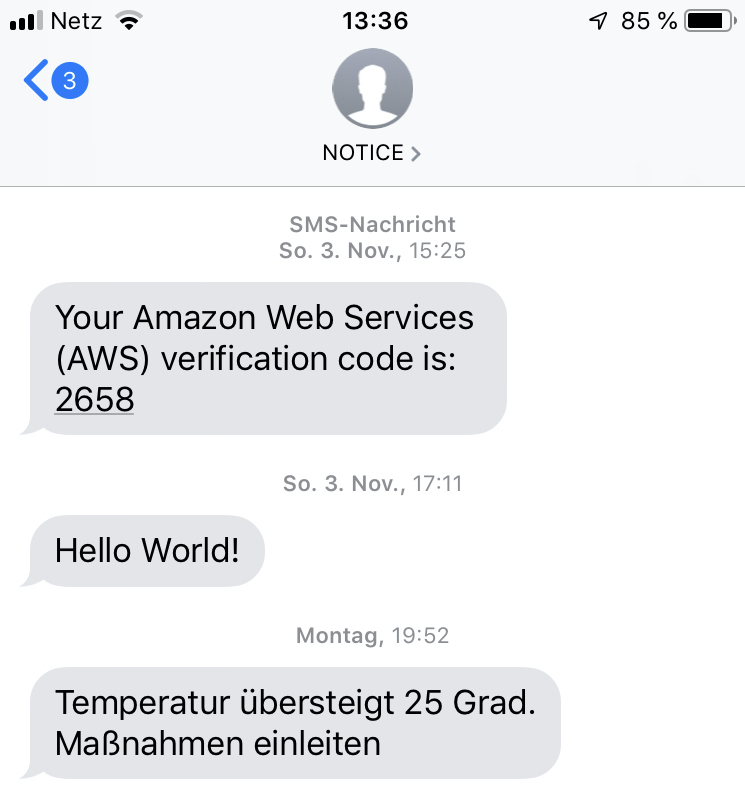
\includegraphics[width=0.6\linewidth]{AWS1_Notification.png}
    \caption{Empfang der Benachrichtigungs-SMS}
    \label{awsnoti}
\end{figure}

% technologische Ebene
\subsection{Evaluation auf technischer Ebene}

Dass die technischen Anforderungen (s. Kapitel \ref{anftechnik}) an den Prototyp größtenteils erfüllt sind, kann damit bestätigt werden, dass der Prototyp auf Systemebene nahezu alle erforderlichen Eigenschaften aufweist. Die funktionalen Anforderungen lassen sich grob in drei Teile aufteilen. Der erste Teil betrifft die Erzeugung eines \ac{cpss} (T-FA-1). Mit der Nutzung eines mit dem Internet verbundenen Raspberry Pi und der Anbindung entsprechender Sensorik wurde ein kommunikationsfähiges und rechnergestütztes System entworfen. Als nächstes wurden Anforderungen an das Gateway definiert  (T-FA-2). Durch die lokale Konfiguration einer Gateway Edge auf Basis des REST-Protokolls wurde eine Industrie-4.0-Komponente erzeugt, indem das physische Medium an ihre Verwaltungsschale angebunden wurde. Das zuverlässige Senden der Messwerte über das Gateway kann bestätigt werden. Auch die Verzögerungen im Empfang der Befehle aus SAP Leonardo IoT sind nicht mit der Unzuverlässigkeit des Gateways, sondern der des Message Processing zu begründen. Als letztes wurden funktionale Anforderungen für die Virtualisierung des \ac{cpss} definiert (T-FA-3). Auch diese Anforderungen erfüllt der Prototyp. Die Messwerte werden zuverlässig vom einem eindeutigen Gateway empfangen, einer \textit{deviceId} zugeordnet und über das Message Processing an den digitalen Zwilling übergeben. Dort werden für die Messwerte, durch die Definition von Regeln und Aktionen, Ereignisse mit den Schweren \textit{High, Medium, Low} (s. Listing \ref{eventex}) generiert. Zudem werden automatische POST-Anfragen an die Web-API des \ac{aws} \ac{sns} gesendet.

\subsection{Handlungsempfehlung}

Die Evaluation des Prototyps ergibt, dass das erzeugte System den Anforderungen des Anwendungsfalls gerecht werden. Da der Prototyp allerdings nur eine Simulation einer Windenergieanlage darstellt, sollte er auf den Fall einer echten Windenergieanlage angewandt werden. Das bedeutet, dass der Auftraggeber Enercon bei einer praktischen Anwendung von SAP Leonardo als Innovationsplattform Anpassungen an der entworfenen Systemarchitektur vornehmen sollte. In der Praxis hat eine Windenergieanlage einen längeren Produktlebenszyklus als in der Simulation dargestellt. Es sollte sichergestellt werden, dass jede Phase, von der Produktion der Einzelteile, über die Installation, bis hin zum Verkauf an den Kunden und dem anschließenden Betrieb, digital abgebildet wird. Dadurch entstehen Herausforderungen, Mechanik und Informationstechnik zusammenzuführen und die Gegenstände sowie alle betroffenen Stakeholder im Lebenszyklus in die Geschäftslogik integrieren. Um dieses mehrdimensionale Netzwerk bewältigen zu können, ist die Orientierung an der \ac{rami} dringend empfohlen. Vor allem, weil die Energiebranche stark von gesetzlichen Regularien abhängt, kann eine Referenz seitens der Regierung die notwendige Flexibilität bieten. Um der Referenzarchitektur gerecht zu werden, sollten die Windenergieanlagen allerdings über OPC-Schnittstellen der \ac{scada}-Systeme in das Industrie"=4.0"=Netzwerk integriert werden. Dies kann durch die Nutzung der \textit{IoT Edge Platform OPC UA} umgesetzt werden (s. Kapitel \ref{datentransport}). Für die horizontale Integration der Anlagen in die Geschäftslogik und Stammdaten sollte die \textit{SAP Cloud Platform Integration} genutzt werden. Wie aus der Ausgangssituation zu entnehmen ist, wird der Auftraggeber auf das ERP-System S/4 HANA umsteigen. Die Nutzung der HANA DB ist dabei dringend empfohlen, damit mit der In-Memory-Technologie die Echtzeitfähigkeit des IoT-Systems gewährleistet werden kann. Mit diesen Maßnahmen können ideale Voraussetzungen entstehen, das Geschäftsfeld von Anlagenbau und -verkauf um digitale Dienstleistungen zu erweitern. Den Kunden können intelligente Anwendungen rund um das Monitoring der Anlagen angeboten werden. Außerdem können durch eine Anbindung der SAP Leonardo Machine Learning Foundation die Wartungs- und Instandhaltungsdienste für die Kunden im Sinne des \textit{Predictive Maintenance} optimiert werden. 
 

\newpage
